\section{Introduction to Stochastic Processes}
We aim to provide a concise introduction to certain classes of stochastic processes, leveraging foundational knowledge of random variables and classical probability theory. To begin, let us recall the concept of conditional probability:
\[
\mathbb{P}(A \mid B) = \frac{\mathbb{P}(A \cap B)}{\mathbb{P}(B)},
\]
provided \( \mathbb{P}(B) > 0 \). This expression can be restructured to compute the probability of an intersection:
\[
\mathbb{P}(A \cap B) = \mathbb{P}(B) \cdot \mathbb{P}(A \mid B).
\]
In the special case of independence, we have:
\[
\mathbb{P}(A \cap B) = \mathbb{P}(A) \cdot \mathbb{P}(B).
\]
Equivalently, \( A \) and \( B \) are independent if the occurrence of \( B \) does not alter the probability of \( A \), i.e., \( \mathbb{P}(A \mid B) = \mathbb{P}(A) \). This highlights that the additional information from \( B \) is irrelevant to our belief about \( A \).

\paragraph{From Random Variables to Stochastic Processes.} 
A random variable \( X \) is a mapping:
\[
X: \Omega \to \mathbb{R},
\]
where \( \Omega \) is the sample space. To incorporate dynamics—phenomena evolving over time—we extend this definition by introducing a time parameter \( t \). Formally, a stochastic process is a function:
\[
X: T \times \Omega \to \mathbb{R},
\]
where \( T \) represents time and \( \Omega \) captures randomness. For a fixed \( t \), \( X(t, \omega) \) is a random variable. For a fixed \( \omega \), \( X(t, \omega) \) describes the path of the process over time. For the sake of notational simplicity, we will use the shorthand \( X_t(\omega) \) to denote \( X(t, \omega) \).


\paragraph{Classification of Stochastic Processes.}
Stochastic processes are broadly categorized based on the nature of \( T \):
\begin{itemize}
    \item Discrete-time stochastic processes: \( T = \mathbb{N} \) (e.g., daily stock prices).
    \item Continuous-time stochastic processes: \( T = [0, \infty) \) (e.g., the motion of particles in a fluid).
\end{itemize}
In discrete time, the process is often represented as a sequence \( \{X_1, X_2, \dots\} \), whereas in continuous time, it is described by a function \( X(t) \) over \( t \in [0, \infty) \).

\paragraph{Perspectives on Stochastic Processes.}
A stochastic process can be viewed in two ways:
\begin{enumerate}
    \item Fixed Time: Fixing \( t \), \( X_t(\omega) \) is a random variable. For instance, observing the price of a stock at a specific time \( t \) treats \( X_t \) as a random variable.
    \item Fixed Outcome: Fixing \( \omega \), \( X_t(\omega) \) describes a path or realization of the process over time. For example, the sequence of outcomes \( X_1(\omega), X_2(\omega), \dots \) might represent the daily movements of a stock.
\end{enumerate}

\paragraph{Continuous-Time Stochastic Processes.}
For continuous time \( T = [0, \infty) \), the paths \( t \mapsto X_t(\omega) \) are often assumed to possess certain regularity properties, such as continuity. A classic example is the Brownian motion, which satisfies:
\begin{itemize}
    \item \( X_t \) for fixed \( t \) is normally distributed.
    \item The paths \( t \mapsto X_t(\omega) \) are continuous but nowhere differentiable.
\end{itemize}
Brownian motion exhibits extreme irregularity, which challenges intuition. While we typically associate continuity with smoothness, most continuous functions (including paths of Brownian motion) are not differentiable. This distinction was rigorously established in the early 20th century.

\paragraph{Implications for Modeling.}
The irregularity of stochastic processes like Brownian motion complicates modeling but is essential for accurately representing phenomena such as stock price fluctuations or particle diffusion. Despite their complexity, these processes provide a robust framework for studying dynamic systems under uncertainty.

\section{Discrete-Time Markov Chains}

\paragraph{Discrete-Time Stochastic Processes.}
We focus exclusively on discrete-time stochastic processes, which are defined as sequences of random variables observed at discrete time points \( t = 0, 1, 2, \dots \). This simplifies the analysis and serves as an excellent starting point for building intuition before tackling more complex cases, such as continuous-time processes. \newline
Rather than considering general stochastic processes in which random variables \( X_n \) take values in \( \mathbb{R} \), we restrict the range to a smaller set \( S \), which is finite or countably infinite. This specific class of processes is called Markov chain.

\paragraph{Definition of a Markov Chain.}
A Markov chain is a stochastic process \( \{X_n\}_{n \geq 0} \), where each random variable \( X_n \) takes values in a set \( S \) (the state space), and the following \textbf{Markov property} holds:
\[
\mathbb{P}(X_{n+1} = x_{n+1} \mid X_0 = x_0, X_1 = x_1, \dots, X_n = x_n) = \mathbb{P}(X_{n+1} = x_{n+1} \mid X_n = x_n),
\]
for all \( x_0, x_1, \dots, x_n, x_{n+1} \in S \). \newline
This property implies that the future state \( X_{n+1} \) depends only on the present state \( X_n \) and is conditionally independent of all past states \( X_0, \dots, X_{n-1} \).

\paragraph{Key Components of a Markov Chain.}
\begin{itemize}
    \item State Space (\( S \)): The set of all possible values the random variables \( X_n \) can take.
    \item Transition Probabilities: The probabilities of moving from one state to another:
  \[
  p_{ij} = \mathbb{P}(X_{n+1} = j \mid X_n = i), \quad i, j \in S.
  \]
  These probabilities are called \textbf{one-step transition probabilities}.
    \item Initial Distribution: The distribution of \( X_0 \), denoted as \( \mathbb{P}(X_0 = i) \) for \( i \in S \). The complete law of the Markov Chain can be obtained if we know the transition probabilities and the initial distributions.
\end{itemize}

\paragraph{Homogeneous Markov Chains.}
A Markov chain is said to be homogeneous if the transition probabilities do not depend on time \( n \). That is:
\[
\mathbb{P}(X_{n+1} = j \mid X_n = i) = p_{ij}, \quad \forall n \geq 0.
\]
In this case, the transition probabilities depend only on the current state \( i \) and the next state \( j \), not on the time \( n \).

\paragraph{Joint Probability Distribution.}
For a Markov chain, the joint probability distribution of the sequence \( X_0, X_1, \dots, X_n \) can be expressed as:
\[
\mathbb{P}(X_0 = x_0, X_1 = x_1, \dots, X_n = x_n) = \mathbb{P}(X_0 = x_0) \prod_{k=0}^{n-1} \mathbb{P}(X_{k+1} = x_{k+1} \mid X_k = x_k).
\]
This formulation highlights that the complete description of the process requires knowledge of:
\begin{enumerate}
    \item The initial distribution \( \mathbb{P}(X_0 = x_0) \).
    \item The transition probabilities \( p_{ij} = \mathbb{P}(X_{n+1} = j \mid X_n = i) \).
\end{enumerate}

\paragraph{Practical Examples of Markov Chains.}
\begin{enumerate}
    \item Random Walk on Integers: A process where \( X_{n+1} = X_n + Y_n \), and \( Y_n \) are independent random variables taking values \( +1 \) or \( -1 \) with equal probability.
    \item Weather Modeling: States represent weather conditions (e.g., sunny, rainy). Transition probabilities capture the likelihood of moving between these states.
    \item Stock Prices: Simplified models of stock price movements, assuming tomorrow's price depends only on today's price.
\end{enumerate}

\section{Markov Chains: Transition Dynamics and Matrix Representation}

\paragraph{Transition Probabilities.}
For a Markov chain, we describe the evolution between states in terms of transition probabilities. Let \( Y \) and \( X \) be states in the state space \( S \). The transition probability from state \( Y \) at time \( n-1 \) to state \( X \) at time \( n \) is denoted as:
\[
P_{YX} = \mathbb{P}(X_n = X \mid X_{n-1} = Y).
\]
For a homogeneous Markov chain, these probabilities are independent of time, so \( P_{YX} \) does not vary with \( n \).

\paragraph{Transition Matrix.}
The collection of transition probabilities can be organized into a transition matrix, denoted by \( P \). Each entry \( P_{YX} \) represents the probability of moving from state \( Y \) to state \( X \). If \( S \) is finite with cardinality \( |S| = N \), then \( P \) is an \( N \times N \) square matrix. For countable \( S \), \( P \) becomes an infinite matrix. \newline
The key properties of a transition matrix are:
\begin{enumerate}
    \item Non-negativity: \( P_{YX} \geq 0 \) for all \( Y, X \in S \).
    \item Row-sum to one: For each state \( Y \in S \),
        \[
        \sum_{X \in S} P_{YX} = 1.
        \]
\end{enumerate}

\paragraph{Example: A Markov Chain with Three States.}
Consider a Markov chain with three states \( S = \{1, 2, 3\} \). The transition matrix \( P \) can be written as:
\[
P = 
\begin{bmatrix}
\frac{1}{2} & \frac{1}{2} & 0 \\
0 & \frac{1}{3} & \frac{2}{3} \\
\frac{1}{3} & \frac{1}{2} & \frac{1}{6}
\end{bmatrix}.
\]
Here:
\begin{itemize}
    \item \( P_{12} = \frac{1}{2} \) is the probability of transitioning from state 1 to state 2.
    \item \( P_{33} = \frac{1}{6} \) is the probability of remaining in state 3.
    \item The rows of \( P \) sum to 1, satisfying the row-sum condition.
\end{itemize}
For the above example:
\begin{itemize}
    \item From state 1, transitions to state 2 and back to state 1 have probabilities \( \frac{1}{2} \) each.
    \item From state 3, transitions to state 1 and state 2 have probabilities \( \frac{1}{3} \) and \( \frac{1}{2} \), respectively.
\end{itemize}

\paragraph{Graphical Representation.}
The transition dynamics can also be represented as a directed graph:
\begin{itemize}
    \item Each state is a node.
    \item Directed edges between nodes indicate possible transitions, labeled with their probabilities.
\end{itemize}

\paragraph{Constructing a Markov Chain.}
A simple method to construct a Markov chain involves:
\begin{enumerate}
    \item An initial random variable \( X_0 \), taking values in \( S \).
    \item A sequence of i.i.d. random variables \( U_1, U_2, \dots \), independent of \( X_0 \).
    \item A function \( F: S \times \mathbb{R} \to S \) that maps the current state and a random input to the next state.
\end{enumerate}
The process is defined recursively:
\[
X_1 = F(X_0, U_1), \quad X_2 = F(X_1, U_2), \quad \dots, \quad X_{n+1} = F(X_n, U_{n+1}).
\]

\paragraph{Verifying the Markov Property.}
To confirm that \( \{X_n\} \) is a Markov chain, we verify that the Markov property holds:
\[
\mathbb{P}(X_{n+1} = x_{n+1} \mid X_n = x_n, X_{n-1} = x_{n-1}, \dots, X_0 = x_0) = \mathbb{P}(X_{n+1} = x_{n+1} \mid X_n = x_n).
\]
Substituting \( X_{n+1} = F(X_n, U_{n+1}) \), we observe that the next state depends only on \( X_n \) and \( U_{n+1} \). Since \( U_1, U_2, \dots \) are i.i.d. and independent of \( X_0 \), the additional conditions \( X_{n-1}, \dots, X_0 \) do not affect the transition probability, confirming the Markov property.

\section{A Special Case of Markov Chains: The Gambler’s Ruin Problem}

\paragraph{Problem Setup.}
Consider a scenario involving two players engaged in a simple gambling game that follows these rules:
\begin{itemize}
    \item The combined wealth of the two players is fixed at \( N \) euros.
    \item Player 1 starts with \( K \) euros, while Player 2 has \( N - K \) euros.
    \item At each step, Player 1 either: 
        \begin{itemize}
            \item Wins \( 1 \) euro with probability \( p \), or
            \item Loses \( 1 \) euro with probability \( 1 - p \).
        \end{itemize}
\end{itemize}

\paragraph{State Evolution.}
Let \( X_n \) represent the money Player 1 has after \( n \) games. The evolution of \( X_n \) can be described as:
\[
X_{n+1} = X_n + U_{n+1},
\]
where \( U_{n+1} \) is a random variable taking the values:
\[
U_{n+1} =
\begin{cases}
+1 & \text{with probability } p, \\
-1 & \text{with probability } 1-p.
\end{cases}
\]
Initial state: \( X_0 = K \), the initial wealth of Player 1.

\paragraph{Boundary Conditions.}
The game is subject to the following rules:
\begin{enumerate}
    \item If \( X_n = 0 \): Player 1 has no money left and is eliminated from the game. The process stops, and \( X_n \) remains at \( 0 \) for all subsequent steps.
    \item If \( X_n = N \): Player 1 has won all the money, and the process stops. \( X_n \) remains at \( N \) for all subsequent steps.
\end{enumerate}

\paragraph{Transition Dynamics.}
The transitions between states can be described by the following rules:
\begin{itemize}
    \item If \( 1 \leq X_n \leq N-1 \):
    \begin{itemize}
        \item Move to \( X_{n+1} = X_n + 1 \) (win) with probability \( p \),
        \item Move to \( X_{n+1} = X_n - 1 \) (lose) with probability \( 1-p \).
    \end{itemize}
    \item If \( X_n = 0 \) or \( X_n = N \), the process remains at that state indefinitely.
\end{itemize}

\paragraph{Transition Matrix Representation.}
The gambler’s ruin problem can be expressed as a Markov chain with \( N+1 \) states \( \{0, 1, \dots, N\} \). The transition matrix \( P \) is given by:
\[
P =
\begin{bmatrix}
1       & 0         & 0      & 0     & 0       & \cdots & 0        & 0      \\
1-p     & 0         & p      & 0     & 0       & \cdots & 0        & 0      \\
0       & 1-p       & 0      & p     & 0       & \cdots & 0        & 0      \\
0       & 0         & 1-p    & 0     & p       & \cdots & 0        & 0      \\
\vdots  & \ddots    & \ddots &\ddots & \ddots  & \ddots & \ddots   & \vdots \\
0       & 0         & 0      & 0     & 0       & 1-p    & 0        & p      \\
0       & 0         & 0      & 0     & 0       & \cdots & 0        & 1      \\
\end{bmatrix},
\]
where:
\begin{itemize}
    \item \( P_{i,i+1} = p \) represents the probability of moving from state \( i \) to \( i+1 \) (winning),
    \item \( P_{i,i-1} = 1-p \) represents the probability of moving from state \( i \) to \( i-1 \) (losing),
    \item \( P_{0,0} = 1 \) and \( P_{N,N} = 1 \) represent absorbing states (no transitions out).
    \item The diagonal entries are \( 0 \), indicating no self-loops.
    \item For all rows, the probabilities sum to \( 1 \), ensuring the matrix is stochastic.
\end{itemize}

\section{Chapman-Kolmogorov Equation}
The Chapman-Kolmogorov equation expresses the relationship between multi-step and single-step transition probabilities in a Markov chain. Let \( P^{(n+m)}_{yx} \) denote the probability of transitioning from state \( y \) to state \( x \) in \( n+m \) steps. This can be written as:
\[
P^{(n+m)}_{yx} = \mathbb{P}(X_{n+m} = x \mid X_0 = y).
\]
To compute \( P^{(n+m)}_{yx} \), we can consider all possible intermediate states \( z \) that the process could occupy after \( n \) steps. This leads to:
\[
P^{(n+m)}_{yx} = \sum_{z \in S} \mathbb{P}(X_{n+m} = x \cap X_n = z \mid X_0 = y).
\]
Using the property of conditional probabilities:
\[
\mathbb{P}(A \cap B) = \mathbb{P}(A \mid B) \cdot \mathbb{P}(B),
\]
we rewrite the probability as:
\[
P^{(n+m)}_{yx} = \sum_{z \in S} \mathbb{P}(X_{n+m} = x \mid X_n = z, X_0 = y) \cdot \mathbb{P}(X_n = z \mid X_0 = y).
\]
By the Markov property, \( \mathbb{P}(X_{n+m} = x \mid X_n = z, X_0 = y) \) depends only on \( z \), not on the full history. Thus:
\[
P^{(n+m)}_{yx} = \sum_{z \in S} P^{(m)}_{zx} \cdot P^{(n)}_{yz}.
\]
In matrix notation, let \( P^{(k)} \) represent the \( k \)-step transition matrix. Then, the Chapman-Kolmogorov equation is expressed as:
\[
P^{(n+m)} = P^{(n)} \cdot P^{(m)}.
\]
The entry in row \( y \), column \( x \) of \( P^{(n+m)} \), denoted \( P^{(n+m)}_{yx} \), is calculated as:
\[
P^{(n+m)}_{yx} = \sum_{z \in S} P^{(n)}_{yz} \cdot P^{(m)}_{zx}.
\]

\paragraph{Key Insights.}
\begin{enumerate}
    \item The probability of transitioning from \( y \) to \( x \) in \( n+m \) steps is obtained by adding all intermediate states \( z \) after \( n \) steps.
    \item The matrix product \( P^{(n+m)} = P^{(n)} \cdot P^{(m)} \) encapsulates this summation.
    \item The Chapman-Kolmogorov equation ensures that the \( k \)-step transition matrices remain stochastic (row sums equal to 1).
\end{enumerate}

\paragraph{Example:}
Consider a Markov chain with the following one-step transition matrix:
\[
P = 
\begin{bmatrix}
\frac{1}{2} & \frac{1}{2} & 0 \\
0 & \frac{1}{3} & \frac{2}{3} \\
\frac{1}{3} & \frac{1}{2} & \frac{1}{6}
\end{bmatrix}.
\]
To compute the two-step transition matrix \( P^2 \), we perform the matrix product \( P \cdot P \):
\[
P^2 = 
\begin{bmatrix}
\frac{1}{2} & \frac{1}{2} & 0 \\
0 & \frac{1}{3} & \frac{2}{3} \\
\frac{1}{3} & \frac{1}{2} & \frac{1}{6}
\end{bmatrix}
\cdot
\begin{bmatrix}
\frac{1}{2} & \frac{1}{2} & 0 \\
0 & \frac{1}{3} & \frac{2}{3} \\
\frac{1}{3} & \frac{1}{2} & \frac{1}{6}
\end{bmatrix}.
\]
The entry \( P^2_{32} \), representing the probability of transitioning from state \( 3 \) to state \( 2 \) in 2 steps, is computed as:
\[
P^2_{32} = \frac{1}{3} \cdot \frac{1}{2} + \frac{1}{2} \cdot \frac{1}{3} + \frac{1}{6} \cdot \frac{1}{2} = \frac{5}{12}.
\]

\paragraph{Important Note.}
\( P^2_{yx} \) is not the square of \( P_{yx} \). It is obtained by summing over all possible intermediate states:
\[
P^2_{yx} = \sum_{z \in S} P_{yz} \cdot P_{zx}.
\]

\paragraph{Distribution of the Process.}
Let \( \mu_y = \mathbb{P}(X_0 = y) \) denote the initial distribution of the process. The distribution of the Markov chain at time \( n \), \( \mathbb{P}(X_n = x) \), can be computed as:
\[
\mathbb{P}(X_n = x) = \sum_{y \in S} \mu_y P^{(n)}_{yx}.
\]
In matrix form:
\[
\mathbf{\mu}^{(n)} = \mathbf{\mu} P^n,
\]
where \( \mathbf{\mu} \) is the row vector of initial probabilities, and \( P^n \) is the \( n \)-step transition matrix.

\paragraph{Classification of States.}
One key goal in studying Markov chains is to classify the states of the process based on their connectivity and recurrence properties. State \( x \) communicates with state \( y \) if there exists a positive probability of transitioning from \( x \) to \( y \) in a finite number of steps, and vice versa.

\section{Example: Sentinel on a Castle}
\begin{center}
    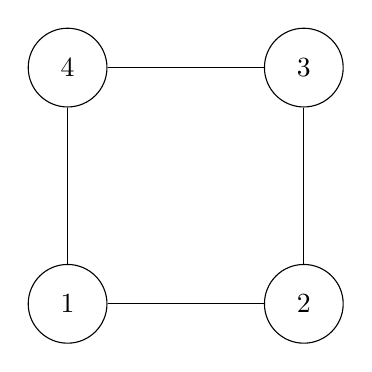
\begin{tikzpicture}[node distance=5cm, every node/.style={circle, draw, minimum size=1cm}]

% Nodes
\node (1) at (0,0) {1};
\node (2) at (3,0) {2};
\node (3) at (0,3) {4};
\node (4) at (3,3) {3};

% Connections
\draw (1) -- (2);
\draw (3) -- (1);
\draw (2) -- (4);
\draw (3) -- (4);

\end{tikzpicture}
\end{center}

Consider a castle with four towers labeled \( 1, 2, 3, 4 \). A sentinel moves between these towers as follows:
\begin{itemize}
    \item At each step, the sentinel flips a coin:
        \begin{itemize}
            \item With probability \( p \), the sentinel moves counterclockwise.
            \item With probability \( 1-p \), the sentinel moves clockwise.
        \end{itemize}
    \item The transition matrix for this system is:
        \[
        P =
        \begin{bmatrix}
        0 & p & 0 & 1-p \\
        1-p & 0 & p & 0 \\
        0 & 1-p & 0 & p \\
        p & 0 & 1-p & 0
        \end{bmatrix}
        \]
    \item Notice that odd-numbered towers (\( 1, 3 \)) and even-numbered towers (\( 2, 4 \)) alternate with each move. It is impossible to transition between two odd or two even towers in a single step.
\end{itemize}

\paragraph{Exercise: Sentinel on a Castle with 5 Towers.}
Now, consider a castle with \( 5 \) towers labeled \( 1, 2, 3, 4, 5 \). 
\begin{center}
    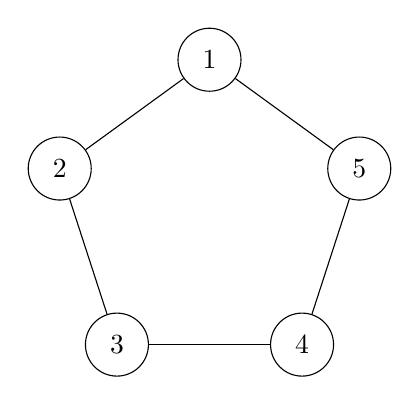
\begin{tikzpicture}[every node/.style={circle, draw, minimum size=0.8cm, inner sep=0pt}]

        % Coordinates for the pentagon's vertices
        \node (1) at (90:2) {1};   % Top point
        \node (2) at (162:2) {2};  % Top-left
        \node (3) at (234:2) {3};  % Bottom-left
        \node (4) at (306:2) {4};  % Bottom-right
        \node (5) at (18:2) {5};   % Top-right

        % Connect outer nodes in a pentagon shape
        \draw (1) -- (2);
        \draw (2) -- (3);
        \draw (3) -- (4);
        \draw (4) -- (5);
        \draw (5) -- (1);

    \end{tikzpicture}
\end{center}
The transition probabilities are defined as:
\begin{itemize}
    \item With probability \( p \), the sentinel moves counterclockwise.
    \item With probability \( 1-p \), the sentinel moves clockwise.
\end{itemize}
The transition matrix for this system is:
\[
P =
\begin{bmatrix}
0 & p & 0 & 0 & 1-p \\
1-p & 0 & p & 0 & 0 \\
0 & 1-p & 0 & p & 0 \\
0 & 0 & 1-p & 0 & p \\
p & 0 & 0 & 1-p & 0
\end{bmatrix}
\]

\paragraph{Analysis.}
\begin{enumerate}
    \item \textbf{Periodicity:}  
    Consider the transitions for a specific tower, say tower \( 1 \). From tower \( 1 \), the sentinel can move to:
    \begin{itemize}
        \item Tower \( 2 \) in one step (clockwise with probability \( p \)).
        \item Tower \( 5 \) in one step (counterclockwise with probability \( 1-p \)).
    \end{itemize}
    To return to tower \( 1 \), the sentinel must traverse all five towers, completing the cycle. The number of steps to return to tower \( 1 \) must be a multiple of \( 5 \). Hence, the period of each tower is \( 5 \), indicating that the system is periodic with a period \( d = 5 \).

    \item \textbf{Connectivity:}  
    From any tower \( i \), the sentinel can reach any other tower \( j \) within at most \( 4 \) steps:
    \begin{itemize}
        \item By moving clockwise, the sentinel transitions through towers \( i+1, i+2, \dots, j \mod 5 \).
        \item By moving counterclockwise, the sentinel transitions through towers \( i-1, i-2, \dots, j \mod 5 \).
    \end{itemize}
    This demonstrates that all towers communicate, and the Markov chain is irreducible.
\end{enumerate}
The system for a sentinel on a 5-tower castle is irreducible and periodic with a period \( d = 5 \). This periodicity means the system does not exhibit ergodic behavior as transitions between states occur only at multiples of the period.


\section{Classification of States in Markov Chains}

\subsection{Communication Between States.}  
The first step in analyzing a Markov chain is to classify the states based on their ability to communicate with each other. 
\begin{enumerate}
    \item Accessibility: State \( j \in S \) is said to be accessible from state \( i \in S \) if there exists a positive integer \( n \) such that the \( (i,j) \)-entry of the \( n \)-step transition matrix \( P^n \), \( (P^n)_{ij} \), satisfies:
\[
(P^n)_{ij} > 0.
\]
This means that there is a positive probability of transitioning from state \( i \) to state \( j \) in exactly \( n \) steps. By convention, \( (P^0)_{ii} = 1 \) for any \( i \in S \), since zero steps correspond to remaining in the same state.
    \item Communication: Two states \( i, j \in S \) communicate if \( j \) is accessible from \( i \), and \( i \) is accessible from \( j \). We denote this relationship by \( i \leftrightarrow j \). The communication relation \( \leftrightarrow \) is an equivalence relation on the state space \( S \). To verify this, we check the following properties:
    \begin{enumerate}
        \item Reflexivity: Any state \( i \) communicates with itself because \( (P^0)_{ii} = 1 \).
        \item Symmetry: If \( i \leftrightarrow j \), then \( j \leftrightarrow i \), as accessibility in one direction implies accessibility in the reverse direction. 
        \item Transitivity: If \( i \leftrightarrow j \) and \( j \leftrightarrow k \), then \( i \leftrightarrow k \). This holds because if there exist \( n \) steps to go from \( i \) to \( j \), and \( m \) steps to go from \( j \) to \( k \), then the probability of transitioning from \( i \) to \( k \) in \( n+m \) steps is:
           \[
           (P^{n+m})_{ik} \geq (P^n)_{ij} \cdot (P^m)_{jk} > 0.
           \]
    \end{enumerate} 
\end{enumerate}

\subsection{Communication Classes.}  
The equivalence relation \( \leftrightarrow \) partitions the state space \( S \) into disjoint subsets called communication classes.  
\begin{itemize}
    \item States within the same communication class can communicate with each other.
    \item States in different classes cannot communicate.
\end{itemize}

\section{Properties of Communication Classes:}
States within the same communication class share key properties, such as:
\begin{itemize}
    \item \textbf{Periodicity:} A state is periodic if it can only be returned to at multiples of a fixed number of steps. The periodicity of a state depends on the set of steps \( n > 0 \) for which \( P_{ii}^n > 0 \) (the probability of returning to state \( i \) in exactly \( n \) steps).For a Markov chain to be aperiodic, at least one state must have \( P_{ii} > 0 \) (self-loops). For example, in a chain where \( P_{11} = \frac{1}{2} \), state \( 1 \) is aperiodic because it can remain in state \( 1 \) for any number of steps, breaking periodicity. A state \( i \) is aperiodic if the greatest common divisor (gcd) of this set is \( 1 \). Otherwise, it is periodic, with the gcd defining its period. \newline 
    For a state \( i \), let:
    \[
    d_i = \gcd\{n > 0 : P_{ii}^n > 0\}.
    \]
        \begin{itemize}
            \item If \( d_i = 1 \), the state is aperiodic.
            \item If \( d_i > 1 \), the state is periodic with period \( d_i \).
        \end{itemize}
    Its properties are:  
        \begin{itemize}
            \item If \( P_{ii} > 0 \), the state \( i \) is automatically aperiodic because it can remain in \( i \) for any number of steps.
            \item If two states \( i \) and \( j \) belong to the same communication class, they share the same periodicity.
        \end{itemize}
     Periodic chains are less desirable in practical applications, as their structured returns can limit randomness and flexibility.

    \item \textbf{Closeness:} A communication class \( C \subseteq S \) is said to be \textbf{closed} if the following holds. For any state \( i \in C \), if state \( j \) is accessible from \( i \), then \( j \) must also belong to \( C \). Formally,  
    \[
    i \in C, \, j \text{ accessible from } i \implies j \in C.
    \]
    This means that it is impossible to leave a closed class and reach states outside it. Once the process enters a closed class, it remains within it forever. 
    
    \item \textbf{Recurrence or Transience:} A state is recurrent if it is visited infinitely often with probability \( 1 \); otherwise, it is transient. If a communication class is not closed, the process will eventually leave it and never return. In the long term, the Markov chain will only visit states in closed classes. Let \( f_i \) be the probability that starting in state \( i \), the Markov chain eventually returns to \( i \):
    \[
    f_i = \mathbb{P}(\exists n \geq 1 \text{ such that } X_n = i \mid X_0 = i).
    \]
        \begin{itemize}
            \item Recurrent State: \( f_i = 1 \). With probability 1, the process will return to \( i \) in a finite amount of time.
            \item Transient State: \( f_i < 1 \). The process may visit \( i \) only a finite number of times.
        \end{itemize}
    Define \( N_i = \#\{n \geq 0 : X_n = i\} \), the number of times the process visits \( i \):  
        \begin{itemize}
            \item If \( i \) is recurrent: \( \mathbb{P}(N_i = \infty \mid X_0 = i) = 1 \).
            \item If \( i \) is transient: \( \mathbb{P}(N_i = \infty \mid X_0 = i) = 0 \).
        \end{itemize}
    Moreover, if \( i \) is transient, \( N_i \) follows a geometric distribution with parameter \( 1-f_i \). \newline
    Also every \textbf{closed class} is a \textbf{recurrent class} and if the state space \( S \) is finite, every recurrent class is closed. Thus, for finite Markov chains, closed classes are equivalent to recurrent classes. In finite-state Markov chains transient states do not significantly affect long-term behavior, as the process eventually leaves them and long-term dynamics are determined entirely by the recurrent classes. \newline 
    Define the expected return time to a state \( i \):
    \[
    m_i = \mathbb{E}[T_i \mid X_0 = i],
    \]
    where \( T_i \) is the first return time to \( i \).  
    \begin{itemize}
        \item A state \( i \) is \textbf{positive recurrent} if \( m_i < \infty \).
        \item A state \( i \) is \textbf{null recurrent} if \( m_i = \infty \).
    \end{itemize}
    
    \item \textbf{Irreducibility:} A Markov chain is called irreducible if all states belong to a single communication class. In other words, every state can communicate with every other state. For irreducible Markov chains:
        \begin{itemize}
            \item All states share the same periodicity.
            \item All states are either recurrent or transient.
        \end{itemize}
    In an irreducible Markov chain, all states share the same periodicity (or aperiodicity).
                
    \item \textbf{Absorbing states:} A state \( i \) is called absorbing if it forms a singleton equivalence class, i.e., once the process enters \( i \), it remains there forever. Due to this they have period equal to 1. 

    \item \textbf{Communication and Recurrence:} if states \( i \) and \( j \) communicate, then
        \begin{itemize}
            \item \( i \) is recurrent if and only if \( j \) is recurrent.
            \item \( i \) is transient if and only if \( j \) is transient.
        \end{itemize}
    
\end{itemize}




\section{Examples of State Classification}
\subsection{Example 1: Transition Matrix}
Consider a Markov chain with state space \( S = \{1, 2, 3\} \) and transition matrix:
\[
P =
\begin{bmatrix}
\frac{1}{2} & \frac{1}{2} & 0 \\
0 & \frac{1}{3} & \frac{2}{3} \\
\frac{1}{3} & 0 & \frac{2}{3}
\end{bmatrix}.
\]
To classify the states:
\begin{enumerate}
    \item Check communication between states:
        \begin{itemize}
           \item From state \( 1 \), it is possible to go to state \( 2 \) in one step (\( P_{12} = \frac{1}{2} > 0 \)).
           \item From state \( 2 \), it is possible to go to state \( 3 \) in one step (\( P_{23} = \frac{2}{3} > 0 \)).
           \item From state \( 3 \), it is possible to return to state \( 1 \) in one step (\( P_{31} = \frac{1}{3} > 0 \)).
   \end{itemize}
    \item Verify symmetry and transitivity: State \( 1 \) is accessible from \( 3 \), state \( 3 \) is accessible from \( 2 \), and state \( 2 \) is accessible from \( 1 \). Thus, all states communicate.
\end{enumerate}

\subsection{Example 2: Sentinel in a Castle.}

Consider the sentinel moving between four towers as described earlier. The state space is \( S = \{1, 2, 3, 4\} \), and the transition probabilities are determined by moving:
\begin{itemize}
    \item Clockwise with probability \( p \).
    \item Counterclockwise with probability \( 1-p \).
\end{itemize}
It is only one communicating class since we can return to every state in a finite number of steps, therefore it is a irreducible MC.

\paragraph{Exercise: Sentinel in a Castle with 5 Towers.}
Now consider a castle with \( 5 \) towers labeled \( S = \{1, 2, 3, 4, 5\} \), and transition probabilities are defined as follows:
\begin{itemize}
    \item With probability \( p \), the sentinel moves clockwise.
    \item With probability \( 1-p \), the sentinel moves counterclockwise.
\end{itemize}
Solution:
\begin{enumerate}
    \item \textbf{Connectivity:}  
    In this system, the sentinel can reach any tower from any other tower within at most \( 4 \) steps, regardless of the starting point. For example:
    \begin{itemize}
        \item Starting from \( 1 \), the sentinel can move to \( 2 \) or \( 5 \) in one step.
        \item From \( 2 \), the sentinel can move to \( 3 \) or \( 1 \), and so on.
    \end{itemize}
    Thus, the system is \textit{irreducible}, as all states communicate with each other.

    \item \textbf{Periodicity:}  
    To determine periodicity, consider the possible number of steps required to return to a specific state, say tower \( 1 \). Starting from \( 1 \):
    \begin{itemize}
        \item It is possible to return to \( 1 \) in \( 5, 10, 15, \dots \) steps.
        \item The greatest common divisor (GCD) of these step counts is \( 5 \).
    \end{itemize}
    Since \( 5 > 1 \), the Markov chain is \textit{periodic} with period \( d = 5 \).

    \item \textbf{Communication Classes:}  
    Since the system is irreducible, all five towers belong to a single communication class:
    \[
    \text{Communication class: } \{1, 2, 3, 4, 5\}.
    \]
\end{enumerate}
For a sentinel moving in a castle with \( 5 \) towers:
\begin{itemize}
    \item The Markov chain is irreducible, as all states communicate.
    \item The Markov chain is periodic, with period \( d = 5 \).
    \item There is a single communication class encompassing all five towers.
\end{itemize}

\subsection{Non-Irreducible Markov Chain Example: Gambler's Ruin}  
Consider the Markov chain representing the classic Gambler's Ruin problem. The state space \( S \) consists of \( M+1 \) states, representing the total money held by two players in a game. At each step:
\begin{itemize}
    \item With probability \( p \), Player A wins 1 euro.
    \item With probability \( 1-p \), Player A loses 1 euro.
\end{itemize}
The state \( X = k \) represents the total amount of money \( k \) held by Player A at a given step. The state space is:
\[
S = \{0, 1, 2, \dots, M\}.
\]
The transition matrix \( P \) is structured as follows:
\begin{itemize}
    \item For \( X = 0 \) (Player A is bankrupt), the process remains in state 0 with probability 1:
    \[
    P_{00} = 1, \quad P_{0j} = 0 \quad \forall j \neq 0.
    \]
    \item For \( X = M \) (Player A has all the money), the process remains in state \( M \) with probability 1:
    \[
    P_{MM} = 1, \quad P_{Mj} = 0 \quad \forall j \neq M.
    \]
    \item For intermediate states \( 1 \leq X \leq M-1 \):
    \[
    P_{k,k+1} = p, \quad P_{k,k-1} = 1-p, \quad P_{kj} = 0 \quad \forall j \notin \{k-1, k+1\}.
    \]
\end{itemize}
Using the definition of communication, the state space can be divided into three equivalence classes:
\begin{itemize}
    \item Class \( \{0\} \): State \( 0 \) is absorbing, meaning once the process enters state \( 0 \), it cannot leave. No other states are accessible from \( 0 \).
    \item Class \( \{M\} \): Similarly, state \( M \) is absorbing. Once the process enters \( M \), it cannot leave.
    \item Class \( \{1, 2, \dots, M-1\} \): The intermediate states communicate with each other since there is a positive probability of transitioning between any pair of states in this range in a finite number of steps. However, states in this class do not communicate with states \( 0 \) or \( M \).
\end{itemize}
\subsection{Example: Sentinel Moving Between Towers}  
Consider a sentinel moving between four towers (states \( 1, 2, 3, 4 \)):
\begin{itemize}
    \item With probability \( p \), the sentinel moves clockwise.
    \item With probability \( 1-p \), the sentinel moves counterclockwise.
\end{itemize}
The transition matrix is:
\[
P =
\begin{bmatrix}
0 & p & 0 & 1-p \\
1-p & 0 & p & 0 \\
0 & 1-p & 0 & p \\
p & 0 & 1-p & 0
\end{bmatrix}.
\]
Starting in state \( 1 \), the sentinel can only return to \( 1 \) after an even number of steps (\( n = 2, 4, 6, \dots \)). The gcd of \( \{n : P_{11}^n > 0\} = \{2, 4, 6, \dots\} \) is \( 2 \). Thus, state \( 1 \) has period \( 2 \). Since all states communicate, the entire Markov chain is periodic with period \( 2 \).
\subsection{Example: Gambler’s Ruin.}  
Consider the Gambler’s Ruin Markov chain with state space \( S = \{0, 1, \dots, M\} \), where:
\begin{itemize}
    \item \( 0 \) and \( M \) are absorbing states.
    \item Intermediate states \( \{1, \dots, M-1\} \) allow transitions with probabilities \( p \) (winning €1) and \( 1-p \) (losing €1).
\end{itemize}
The equivalence classes are:  
\begin{enumerate}
    \item \( C_0 = \{0\} \): The absorbing state \( 0 \). From \( 0 \), there are no transitions to any other state. Hence, \( C_0 \) is a closed class.
    \item \( C_M = \{M\} \): The absorbing state \( M \). Similarly, \( C_M \) is a closed class.
    \item \( C_2 = \{1, \dots, M-1\} \): The transient states. From any state \( i \in C_2 \), there is a nonzero probability of reaching either \( 0 \) or \( M \), which are outside \( C_2 \). Hence, \( C_2 \) is not closed.
\end{enumerate}
\section{Analysis of Random Walks}
\paragraph{Example: Random Walk on \( \mathbb{Z} \).}  
Consider a random walk on the integer lattice \( \mathbb{Z} \) where at each step, the process moves forward with probability \( p \) or backward with probability \( 1-p \).  \newline
The Markov chain is defined as:  
\[
S_{n+1} = S_n + X_{n+1}, \quad X_n \sim \begin{cases} 
1 & \text{with probability } p, \\ 
-1 & \text{with probability } 1-p. 
\end{cases}
\]  
Every state \( i \in \mathbb{Z} \) communicates with every other state. Any state can be reached from any other state in a finite number of steps. Since the state space is infinite, recurrence depends on the probabilities \( p \) and \( 1-p \). There are some special sases: 
\begin{enumerate}
    \item If \( p = 1 \): The process moves deterministically forward, and all states are transient.
    \item If \( p = 0 \): The process moves deterministically backward, and all states are transient.
    \item If \( 0 < p < 1 \): The random walk is irreducible, and all states communicate. However, whether the states are recurrent or transient depends on further analysis of the walk's behavior.
\end{enumerate}
In finite state spaces, the distinction between recurrent and transient states aligns perfectly with the closed or non-closed classification of communication classes. For infinite state spaces, additional considerations are required to determine recurrence, especially for processes like random walks.

\subsection{Random walks} 
Consider a sequence of independent and identically distributed (i.i.d.) random variables \( X_1, X_2, \ldots \) where:  
\[
X_k = 
\begin{cases} 
1 & \text{with probability } P, \\
-1 & \text{with probability } 1-P. 
\end{cases}
\]  
We are interested in the properties of the random walk \( S_n \) defined as:
\[
S_n = S_0 + X_1 + X_2 + \ldots + X_n, \quad \text{where } S_0 \text{ is the initial position.}
\]  
The expectation of \( X_k \) is given by:  
\[
\mathbb{E}[X_k] = P \cdot 1 + (1-P) \cdot (-1) = 2P - 1.
\]
By the strong law of large numbers:  
\[
\frac{S_n}{n} \xrightarrow{\text{a.s.}} \mathbb{E}[X_k] = 2P - 1 \quad \text{as } n \to \infty.
\]  
This implies:  
\begin{itemize}
    \item If \( P > \frac{1}{2} \), \( 2P - 1 > 0 \) and \( S_n \to +\infty \) almost surely.
    \item If \( P < \frac{1}{2} \), \( 2P - 1 < 0 \) and \( S_n \to -\infty \) almost surely.
    \item If \( P = \frac{1}{2} \), the random walk is symmetric, and \( \frac{S_n}{n} \to 0 \) almost surely.
\end{itemize}

\paragraph{Case \( P > \frac{1}{2} \) or \( P < \frac{1}{2} \).}  
In these cases since \( S_n \to \pm\infty \), the state \( 0 \) is \textbf{transient}. A transient state implies that the probability of returning to \( 0 \) infinitely often is zero.

\paragraph{Case \( P = \frac{1}{2} \) (Symmetric Random Walk).}  
For the symmetric random walk:  
\[
\mathbb{E}[X_k] = 0 \quad \text{and} \quad \frac{S_n}{n} \to 0 \quad \text{almost surely.}
\]  
Here, we determine whether the state \( 0 \) is \textbf{recurrent} or \textbf{transient}.  

\paragraph{Recurrence and Transience Criterion.}  
The state \( 0 \) is recurrent if and only if:  
\[
\sum_{n=0}^\infty P^n_{00} = \infty,
\]  
where \( P^n_{00} \) is the probability of returning to \( 0 \) in \( n \) steps. Otherwise, \( 0 \) is transient.

\paragraph{Transition Probabilities.}  
The probability of returning to \( 0 \) in \( n \) steps depends on the number of forward (\(+1\)) and backward (\(-1\)) steps. For \( n \) steps, let \( J \) be the number of forward steps. To return to \( 0 \), the number of forward and backward steps must satisfy:  
\[
J = \frac{n}{2}.
\]  
This is only possible if \( n \) is even. Let \( n = 2J \).  \newline
The probability of \( J \) forward steps and \( J \) backward steps in \( n \) total steps is:  
\[
P^n_{00} = \binom{2J}{J} P^J (1-P)^J.
\]  
For the symmetric random walk (\( P = \frac{1}{2} \)):  
\[
P^n_{00} = \binom{2J}{J} \left(\frac{1}{2}\right)^{2J}.
\]

\paragraph{Summation of Transition Probabilities.}  
We sum \( P^n_{00} \) over all even \( n = 2J \):  
\[
\sum_{n=0}^\infty P^n_{00} = \sum_{J=0}^\infty \binom{2J}{J} \left(\frac{1}{2}\right)^{2J}.
\]  

\paragraph{Stirling's Formula.}  
Stirling's approximation provides an asymptotic formula for \( n! \) as \( n \to \infty \):
\[
n! \sim n^n e^{-n} \sqrt{2 \pi n}.
\]
If we divide \( n! \) by this approximation and take the limit as \( n \to \infty \), we obtain:
\[
\lim_{n \to \infty} \frac{n!}{n^n e^{-n} \sqrt{2 \pi n}} = 1.
\]
This allows us to replace factorial terms with their approximations in series, preserving convergence properties.

\paragraph{Application to Transition Probabilities.}  
For the symmetric random walk (\( P = \frac{1}{2} \)), the probability of returning to \( 0 \) in \( 2J \) steps is given by:
\[
P_{00}^{2J} = \binom{2J}{J} \left(\frac{1}{2}\right)^{2J}.
\]
Using Stirling's formula, we approximate:
\[
\binom{2J}{J} = \frac{(2J)!}{(J!)^2} \sim \frac{(2J)^{2J} e^{-2J} \sqrt{2 \pi (2J)}}{\left(J^J e^{-J} \sqrt{2 \pi J}\right)^2}.
\]
Substituting this into the expression for \( P_{00}^{2J} \), we simplify:
\[
P_{00}^{2J} \sim \frac{(2J)^{2J} e^{-2J} \sqrt{2 \pi (2J)}}{\left(J^J e^{-J} \sqrt{2 \pi J}\right)^2} \cdot \left(\frac{1}{2}\right)^{2J}.
\]
Simplify term by term:
\begin{itemize}
    \item The \( e^{-2J} \) in the numerator cancels with \( e^{-2J} \) in the denominator.
    \item The factorial terms simplify as:
\[
\frac{(2J)^{2J}}{J^{2J}} = 2^{2J}.
\]
    \item Combining the square root terms:
\[
\frac{\sqrt{2 \pi (2J)}}{2 \pi J} = \frac{\sqrt{2}}{\sqrt{\pi J}}.
\]
\end{itemize}
Thus:
\[
P_{00}^{2J} \sim \frac{4^J}{\sqrt{\pi J}} \cdot \left(\frac{1}{4}\right)^J = \frac{1}{\sqrt{\pi J}}.
\]

\paragraph{Summation of Transition Probabilities.}  
To determine recurrence, we sum over all even \( n = 2J \):
\[
\sum_{n=0}^\infty P_{00}^n \sim \sum_{J=1}^\infty \frac{1}{\sqrt{\pi J}}.
\]
The series \( \sum_{J=1}^\infty \frac{1}{\sqrt{J}} \) diverges, indicating that the state \( 0 \) is \textbf{recurrent}.

\paragraph{Extension to Higher Dimensions.}  
For a symmetric random walk in higher dimensions:  
\begin{itemize}
    \item In 1D, the return probability is proportional to \( \frac{1}{\sqrt{n}} \), and the series diverges, indicating recurrence.
    \item In 2D, the return probability is proportional to \( \frac{1}{n} \), and the harmonic series diverges, also indicating recurrence.
    \item In 3D, the return probability is proportional to \( \frac{1}{n^{3/2}} \), and the series converges, indicating transience.
\end{itemize}





\section{Theorem on Ergodic Markov Chains}
A state \( i \) is \textbf{ergodic} if it is aperiodic and positive recurrent. A Markov chain is \textbf{ergodic} if all its states are ergodic. Ergodic Markov chains are foundational for applications in fields such as machine learning and physics.
\paragraph{Theorem.}  
Let \( X_n \) be an irreducible and ergodic Markov chain with state space \( S \). Then:  
\begin{enumerate}
    \item For each \( j \in S \), there exists a limit:
   \[
   \lim_{n \to \infty} P_{ij}^{(n)} = \pi_j,
   \]
   where the limit \( \pi_j \) is independent of the initial state \( i \).  
   Hence, as \( n \to \infty \), the \( (i, j) \)-entry of the transition probability matrix \( P^{(n)} \) converges to \( \pi_j \), and this holds for any initial state \( i \).  
    \item The limiting distribution \( \pi = (\pi_j)_{j \in S} \) is the unique solution to the system:
   \[
   \pi = \pi P, \quad \sum_{j \in S} \pi_j = 1,
   \]
   where \( P \) is the transition matrix of the Markov chain. This implies that \( \pi \) is a probability distribution.
\end{enumerate}
The values \( \pi_j \) represent the \emph{long-term probabilities} of finding the Markov chain in state \( j \), regardless of the initial state \( i \). The distribution \( \pi \) is called the \emph{stationary distribution} or \emph{invariant distribution}. It satisfies:
   \[
   \pi P = \pi,
   \]
   meaning that the distribution remains unchanged after applying the transition matrix.

\paragraph{Properties of \( \pi \):}  
\begin{enumerate}
    \item For each \( j \in S \), \( \pi_j \) can be expressed as:
   \[
   \pi_j = \frac{1}{m_j},
   \]
   where \( m_j \) is the expected return time to state \( j \) (i.e., the average number of steps required to return to \( j \) starting from \( j \)).  
   Since \( m_j > 0 \), it follows that \( \pi_j > 0 \) for all \( j \).
   \item The limiting proportion of time spent in state \( j \) is given by:
   \[
   \pi_j = \lim_{n \to \infty} \frac{\text{Number of visits to } j \text{ by time } n}{n}.
   \]
   This means \( \pi_j \) quantifies how often the chain visits state \( j \) in the long run.
\end{enumerate}

\paragraph{Stationary Distribution and Initial Distribution.}  
If the initial state \( X_0 \) is distributed according to \( \pi \), then the distribution of \( X_n \) remains invariant for all \( n \), i.e.,:
\[
\mathbb{P}(X_0 = i) = \pi_i \quad \implies \quad \mathbb{P}(X_n = i) = \pi_i, \quad \forall n \geq 0.
\]
This property shows that the Markov chain is in \emph{statistical equilibrium} when it starts from the stationary distribution.

\paragraph{Matrix Interpretation.}  
In terms of linear algebra, \( \pi \) is a left eigenvector of the matrix \( P \) corresponding to the eigenvalue \( 1 \):
   \[
   \pi P = \pi.
   \]
If \( S \) is finite, \( P \) is a stochastic matrix, and it is straightforward to prove that \( 1 \) is an eigenvalue. Solving \( \pi P = \pi \) with the normalization \( \sum_{j} \pi_j = 1 \) yields a unique stationary distribution.

\paragraph{Example.}  
Consider the Markov chain with transition matrix:
\[
P = 
\begin{bmatrix}
\frac{1}{2} & \frac{1}{2} & 0 \\
0 & \frac{1}{3} & \frac{2}{3} \\
\frac{1}{3} & \frac{1}{2} & \frac{1}{6}
\end{bmatrix}.
\]
This Markov chain is irreducible and aperiodic (since all states communicate and there are non-zero diagonal entries). Thus, there exists a unique stationary distribution \( \pi = (\pi_1, \pi_2, \pi_3) \) satisfying:
\[
\pi = \pi P, \quad \pi_1 + \pi_2 + \pi_3 = 1.
\]
Expanding \( \pi P = \pi \) gives the system:
\[
\begin{aligned}
    \frac{1}{2} \pi_1 + \frac{1}{3} \pi_3 &= \pi_1, \\
    \frac{1}{2} \pi_1 + \frac{1}{3} \pi_2 + \frac{1}{2} \pi_3 &= \pi_2, \\
    \frac{2}{3} \pi_2 + \frac{1}{6} \pi_3 &= \pi_3.
\end{aligned}
\]
Adding the normalization condition \( \pi_1 + \pi_2 + \pi_3 = 1 \), we solve to obtain:
\[
\pi_1 = \frac{8}{35}, \quad \pi_2 = \frac{15}{35}, \quad \pi_3 = \frac{12}{35}.
\]

\section{Reversible Markov Chains}
A special class of Markov chains is the \textit{reversible Markov chains}, which admit a specific structure for their stationary distribution.

\paragraph{Definition.}
Let \( P \) be the transition matrix of a Markov chain, and let \( \pi \) be a probability distribution on \( S \). We say that \( \pi \) is \textit{reversible} for \( P \) if, for all \( x, y \in S \),
\[
\pi(x) P(x, y) = \pi(y) P(y, x).
\]

\paragraph{Remarks.}
\begin{itemize}
    \item This condition is trivial when \( x = y \) because it reduces to:
    \[
    \pi(x) P(x, x) = \pi(x) P(x, x),
    \]
    which holds automatically.
    \item The condition must be checked only for \( x \neq y \).
    \item If \( \pi \) is constant (uniform distribution), this condition holds if and only if \( P \) is a symmetric matrix:
    \[
    P(x, y) = P(y, x), \quad \forall x, y \in S.
    \]
\end{itemize}

\paragraph{Detailed Balance Condition.}
The equation \( \pi(x) P(x, y) = \pi(y) P(y, x) \) is called the \textit{detailed balance condition}. When \( \pi \) satisfies this condition, \( \pi \) and \( P \) are said to be in \textit{detailed balance}.

\paragraph{Proposition.}
If \( \pi \) satisfies the detailed balance condition:
\[
\pi(x) P(x, y) = \pi(y) P(y, x), \quad \forall x, y \in S,
\]
then \( \pi \) is a stationary distribution for \( P \), i.e.,
\[
\pi = \pi P.
\]

\paragraph{Proof.}
To show \( \pi = \pi P \), consider the \( x \)-th component of \( \pi P \):
\[
(\pi P)(x) = \sum_{y \in S} \pi(y) P(y, x).
\]
By the detailed balance condition, we have \( \pi(y) P(y, x) = \pi(x) P(x, y) \). Substituting:
\[
\sum_{y \in S} \pi(y) P(y, x) = \sum_{y \in S} \pi(x) P(x, y).
\]
Factoring out \( \pi(x) \):
\[
\sum_{y \in S} \pi(y) P(y, x) = \pi(x) \sum_{y \in S} P(x, y).
\]
Since \( P \) is a stochastic matrix, \( \sum_{y \in S} P(x, y) = 1 \), so:
\[
(\pi P)(x) = \pi(x),
\]
and hence \( \pi = \pi P \).

\section{Double Stochastic Matrices}

A \textbf{double stochastic matrix} is defined as a matrix \( P \) such that:
\[
\sum_x P_{xy} = 1 \quad \text{for all } y \in S,
\]
in addition to the standard condition of a stochastic matrix, \( \sum_y P_{xy} = 1 \quad \forall x \in S \).

\paragraph{Invariant Distribution for Double Stochastic Matrices}
\begin{itemize}
    \item If \( S \) is finite, and the transition matrix \( P \) is double stochastic, the uniform distribution \( \pi_i = \frac{1}{|S|} \) is always an invariant distribution.
    \item To check whether a stochastic matrix \( P \) is double stochastic:
        \begin{enumerate}
            \item Verify if the sum of each column is equal to 1.
            \item If this condition holds, the uniform distribution is the invariant distribution.
        \end{enumerate}
\end{itemize}

\paragraph{Proof of Invariance for Uniform Distribution}
Let \( \pi_i = \frac{1}{|S|} \). For \( P \) to admit \( \pi \) as an invariant distribution:
\[
\pi P = \pi.
\]
The \( x \)-th component of \( \pi P \) is given by:
\[
\sum_y \pi_y P_{yx}.
\]
Since \( \pi_y = \frac{1}{|S|} \), this becomes:
\[
\pi_x = \frac{1}{|S|} \sum_y P_{yx}.
\]
If \( P \) is double stochastic, \( \sum_y P_{yx} = 1 \), so:
\[
\pi_x = \frac{1}{|S|}.
\]
Thus, \( \pi \) remains invariant under the application of \( P \).
\section{Examples}
\subsection{Simple Case: Markov Chain with Two States}

The simplest case of a Markov chain arises when the state space \( S \) consists of only two states. Let us label these states \( 0 \) and \( 1 \) (or alternatively \( A \) and \( B \)). The transition matrix for this system is defined as follows:
\[
P =
\begin{bmatrix}
1 - p & p \\
q & 1 - q
\end{bmatrix},
\]
where \( p \) and \( q \) are the transition probabilities ($p,q \in [0,1]$).

\paragraph{Properties of the Transition Matrix}
\begin{itemize}
    \item \( p \) represents the probability of transitioning from state \( 0 \) to state \( 1 \).
    \item \( q \) represents the probability of transitioning from state \( 1 \) to state \( 0 \).
    \item The off-diagonal elements of the matrix, \( p \) and \( q \), are independent constants such that \( 0 < p, q < 1 \). 
    \item The diagonal elements \( 1 - p \) and \( 1 - q \) represent the probabilities of remaining in the same state.
\end{itemize}

\paragraph{Irreducibility}
The Markov chain is \textit{irreducible} if and only if both transitions between states are possible, i.e., \( p > 0 \) and \( q > 0 \). 
\begin{itemize}
    \item If \( p = 0 \), the chain cannot transition from \( 0 \) to \( 1 \), making \( 0 \) an absorbing state.
    \item Similarly, if \( q = 0 \), the chain cannot transition from \( 1 \) to \( 0 \), making \( 1 \) an absorbing state.
    \item If either \( p \) or \( q \) equals \( 0 \), the chain is not irreducible because there are no two-way transitions between the states.
    \item If \( p = q = 0 \), the matrix \( P \) becomes the identity matrix:
    \[
    P =
    \begin{bmatrix}
    1 & 0 \\
    0 & 1
    \end{bmatrix}.
    \]
    In this case, both states \( 0 \) and \( 1 \) are absorbing, and the chain remains forever in its initial state.
    \item If \( P \) is irreducible, there exists a unique invariant distribution, which we compute as follows.
\end{itemize}

\paragraph{Invariant Distribution}
The invariant distribution \( \pi = (\pi_0, \pi_1) \) satisfies the system:
\[
\pi = \pi P \quad \text{and} \quad \pi_0 + \pi_1 = 1.
\]
This can be rewritten as:
\[
\begin{cases}
\pi_0 (1 - p) + \pi_1 q = \pi_0, \\
\pi_0 p + \pi_1 (1 - q) = \pi_1.
\end{cases}
\]
Simplifying the first equation:
\[
\pi_1 q = \pi_0 p.
\]
From this, we derive the ratio:
\[
\pi_1 = \frac{p}{q} \pi_0.
\]
Using the normalization condition \( \pi_0 + \pi_1 = 1 \), we substitute \( \pi_1 = \frac{p}{q} \pi_0 \):
\[
\pi_0 + \frac{p}{q} \pi_0 = 1.
\]
Factoring out \( \pi_0 \):
\[
\pi_0 \left( 1 + \frac{p}{q} \right) = 1.
\]
\[
\pi_0 = \frac{q}{p + q}.
\]
Similarly, substituting for \( \pi_1 \):
\[
\pi_1 = \frac{p}{p + q}.
\]
Thus, the unique invariant distribution is:
\[
\pi = \left( \frac{q}{p+q}, \frac{p}{p+q} \right).
\]

\paragraph{Special Observations}
\begin{itemize}
    \item If \( p = 0 \), we have \( \pi = (1, 0) \), meaning the chain remains in state \( 0 \).
    \item If \( q = 0 \), we have \( \pi = (0, 1) \), meaning the chain remains in state \( 1 \).
    \item For irreducible chains (\( p > 0, q > 0 \)), both \( \pi_0 \) and \( \pi_1 \) are strictly positive.
\end{itemize}

\paragraph{Reversible Distribution}
The detailed balance equation for reversibility is:
\[
\pi_0 P_{01} = \pi_1 P_{10}.
\]
Substituting \( \pi_0 = \frac{q}{p+q} \), \( \pi_1 = \frac{p}{p+q} \), \( P_{01} = p \), and \( P_{10} = q \):
\[
\frac{q}{p+q} p = \frac{p}{p+q} q.
\]
Both sides are equal, confirming that the chain is reversible.

\subsection{Example: Sentinel Case in a Reversible Markov Chain}

\paragraph{Transition Matrix}
Consider a Markov chain where the transition matrix \( P \) is defined as:
\[
P =
\begin{bmatrix}
0 & \frac{1}{2} & 0 & \frac{1}{2} \\
\frac{1}{2} & 0 & \frac{1}{2} & 0 \\
0 & \frac{1}{2} & 0 & \frac{1}{2} \\
\frac{1}{2} & 0 & \frac{1}{2} & 0
\end{bmatrix}.
\]
This Markov chain is:
\begin{itemize}
    \item \textbf{Irreducible:} Every state communicates with every other state.
    \item \textbf{Reversible:} The detailed balance condition holds.
\end{itemize}
These properties ensure the existence of a unique invariant distribution.

\paragraph{Invariant Distribution}
For any irreducible and reversible Markov chain with a finite state space \( S \), there exists a unique invariant distribution. \newline
Applying the detailed balance equations:
\[
\pi_x P_{xy} = \pi_y P_{yx}, \quad \forall x, y \in S, \ x \neq y,
\]
we verify the following:
\begin{itemize}
    \item For states \( 1, 2, 3, \) and \( 4 \), the probabilities \( P_{xy} = \frac{1}{2} \) for connected pairs.
    \item Using symmetry, \( \pi_1 = \pi_2 = \pi_3 = \pi_4 \).
\end{itemize}
Since \( \pi \) must be a probability distribution:
\[
\pi_1 + \pi_2 + \pi_3 + \pi_4 = 1,
\]
we conclude:
\[
\pi_1 = \pi_2 = \pi_3 = \pi_4 = \frac{1}{4}.
\]
Thus, the invariant distribution is:
\[
\pi = \left( \frac{1}{4}, \frac{1}{4}, \frac{1}{4}, \frac{1}{4} \right).
\]
\paragraph{Special Property of the Matrix}
This matrix \( P \) exhibits a unique structure:
\begin{itemize}
    \item It is a \textbf{stochastic matrix}, meaning that the sum of each row equals \( 1 \).
    \item It is also \textbf{doubly stochastic}, meaning that the sum of each column equals \( 1 \).
\end{itemize}
\textbf{Implication:} For doubly stochastic matrices, the uniform distribution is always an invariant distribution.



\subsection{Example: Ehrenfest Model}
The Ehrenfest model, introduced by German mathematician Paul Ehrenfest, is a simple Markov chain that models the random movement of molecules between two containers.
\begin{itemize}
    \item Assume there are two containers, labeled Box 1 and Box 2.
    \item There are \( M \) molecules in total.
    \item Define \( X_n \) as the number of molecules in Box 1 at time \( n \).
\end{itemize}
The state space \( S \) is \( \{0, 1, 2, \dots, M\} \), where \( X_n = i \) indicates that \( i \) molecules are in Box 1 at time \( n \). At each time step:
\begin{enumerate}
    \item A molecule is chosen uniformly at random from all \( M \) molecules.
    \item The chosen molecule is moved from its current box to the other box.
\end{enumerate}

\paragraph{Transition Probabilities}
\begin{itemize}
    \item From state \( i \), the number of molecules in Box 1 can increase to \( i+1 \) if a molecule from Box 2 is moved to Box 1:
    \[
    P(i \to i+1) = \frac{M-i}{M}.
    \]
    \item Similarly, the number of molecules in Box 1 can decrease to \( i-1 \) if a molecule from Box 1 is moved to Box 2:
    \[
    P(i \to i-1) = \frac{i}{M}.
    \]
    \item At the boundaries:
        \begin{itemize}
            \item If \( i = 0 \), \( P(0 \to 1) = 1 \) and it always transitions to \( i = 1 \) (Box 1 is empty, so a molecule is always added).
            \item If \( i = M \), \( P(M \to M-1) = 1 \) and it always transitions to \( i = M-1 \) (Box 1 is full, so a molecule is always removed).
        \end{itemize}
\end{itemize}


\paragraph{Invariant Distribution}
The Ehrenfest model is an irreducible Markov chain. Since \( S \) is finite, there exists a unique invariant distribution. Using the detailed balance equation, it can be shown that:
\[
\pi_i = \binom{M}{i} \frac{1}{2^M},
\]
where \( \pi \) follows a binomial distribution with parameters \( M \) and \( \frac{1}{2} \):
\[
\pi \sim \text{Binomial}(M, \frac{1}{2}).
\]

\paragraph{Interpretation}
\begin{itemize}
    \item If the initial number of molecules in Box 1 is distributed as \( \text{Binomial}(M, \frac{1}{2}) \), the distribution remains invariant over time.
    \item This reflects the long-term equilibrium of the system, where the expected number of molecules in Box 1 is \( \frac{M}{2} \).
\end{itemize}


\subsection{Random Walk on an Undirected Graph}

\paragraph{Definition and Setup}
Consider a random walker on an undirected, connected graph \( G = (V, E) \), where:
\begin{itemize}
    \item \( V = \{1, 2, \dots, N\} \) represents the set of vertices.
    \item \( E \) is the set of edges connecting the vertices.
\end{itemize}
The graph is undirected, meaning movement between vertices is bidirectional, i.e., if there is an edge between \( i \) and \( j \), the walker can move from \( i \) to \( j \) and vice versa with positive probability.

\paragraph{Random Walk Dynamics:}
At each step:
\begin{itemize}
    \item If the walker is at vertex \( i \), it moves to one of its neighbors \( j \) chosen uniformly at random.
    \item The transition probability from \( i \) to \( j \) is:
    \[
    P(i \to j) =
    \begin{cases}
    \frac{1}{\text{deg}(i)} & \text{if } (i, j) \in E, \\
    0 & \text{otherwise},
    \end{cases}
    \]
    where \( \text{deg}(i) \) is the degree of vertex \( i \), i.e., the number of edges connected to \( i \).
\end{itemize}

\paragraph{Transition Matrix}
The transition matrix \( P \) is defined as:
\[
P_{ij} =
\begin{cases}
\frac{1}{\text{deg}(i)} & \text{if } (i, j) \in E, \\
0 & \text{otherwise}.
\end{cases}
\]

\paragraph{Example Graph}
Consider a graph with 5 vertices connected as follows:
\begin{center}
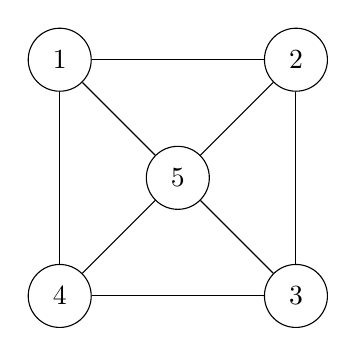
\begin{tikzpicture}[node distance=2cm, every node/.style={circle, draw, minimum size=0.8cm, inner sep=0pt}]
    % Define nodes
    \node (center) at (0,0) {5};
    \node (topLeft) at (-1.5,1.5) {1};
    \node (topRight) at (1.5,1.5) {2};
    \node (bottomRight) at (1.5,-1.5) {3};
    \node (bottomLeft) at (-1.5,-1.5) {4};

    % Draw edges from center to corners
    \draw (center) -- (topLeft);
    \draw (center) -- (topRight);
    \draw (center) -- (bottomRight);
    \draw (center) -- (bottomLeft);

    % Draw edges between corner nodes
    \draw (topLeft) -- (topRight);
    \draw (topRight) -- (bottomRight);
    \draw (bottomRight) -- (bottomLeft);
    \draw (bottomLeft) -- (topLeft);
\end{tikzpicture}
\end{center}
The degrees of the vertices are:
\[
\text{deg}(1) = 3, \quad \text{deg}(2) = 3, \quad \text{deg}(3) = 3, \quad \text{deg}(4) = 3, \quad \text{deg}(5) = 4.
\]
The transition probabilities for vertex \( i \) to \( j \) are \( P_{ij} = \frac{1}{\text{deg}(i)} \) for connected vertices and the transition matrix \( P \) for the random walk is given by:
\[
P =
\begin{bmatrix}
0 & \frac{1}{3} & 0 & \frac{1}{3} & \frac{1}{3} \\
\frac{1}{3} & 0 & \frac{1}{3} & 0 & \frac{1}{3} \\
0 & \frac{1}{3} & 0 & \frac{1}{3} & \frac{1}{3} \\
\frac{1}{3} & 0 & \frac{1}{3} & 0 & \frac{1}{3} \\
\frac{1}{4} & \frac{1}{4} & \frac{1}{4} & \frac{1}{4} & 0
\end{bmatrix}.
\]
If we define \(\xi_i\) as the number of neighbors of a vertex \(i\), then:
\begin{itemize}
    \item For vertices \(i = 1, 2, 3, 4\), \(\xi_i = 3\). For example, vertex 1 can move to vertices 2, 4, and 5.
    \item For vertex 5, \(\xi_5 = 4\).
\end{itemize}
If we denote \(X\) as the total number of neighbors, we have:
\[
X = \xi_1 + \xi_2 + \xi_3 + \xi_4 + \xi_5 = 3 + 3 + 3 + 3 + 4 = 16.
\]
Next, let us define \(\pi_i\) as:
\[
\pi_i = \frac{\xi_i}{X}.
\]
This represents a probability distribution. For any two connected vertices \(i\) and \(j\), the following equality holds:
\[
\pi_i P_{ij} = \pi_j P_{ji}.
\]
\paragraph{Verification:}
\begin{itemize}
    \item If \(P_{ij} \neq 0\), the probability of transitioning from \(i\) to \(j\) is:
    \[
    P_{ij} = \frac{1}{\xi_i}.
    \]
    Similarly, \(P_{ji} = \frac{1}{\xi_j}\).
    \item Using \(\pi_i = \frac{\xi_i}{X}\) and \(\pi_j = \frac{\xi_j}{X}\), it follows:
    \[
    \pi_i P_{ij} = \frac{\xi_i}{X} \cdot \frac{1}{\xi_i} = \frac{1}{X}.
    \]
    Similarly:
    \[
    \pi_j P_{ji} = \frac{\xi_j}{X} \cdot \frac{1}{\xi_j} = \frac{1}{X}.
    \]
    Hence, \(\pi_i P_{ij} = \pi_j P_{ji}\).
\end{itemize}
This property demonstrates that \(\pi = (\pi_1, \pi_2, \dots, \pi_N)\) is the invariant distribution of the Markov chain.

\subsection{Random Walks on a Chessboard}
Consider a knight moving randomly on an \(8 \times 8\) chessboard. The movement of a knight follows an L-shape: two squares in one direction and one perpendicular. The number of neighbors depends on the knight's position:
\begin{itemize}
    \item At a corner (e.g., square \((1,1)\)): \(2\) possible moves.
    \item At an edge but not a corner: \(3\) possible moves.
    \item At the center: \(8\) possible moves.
\end{itemize}
The invariant distribution \(\pi_{ij}\) for any square \((i,j)\) is proportional to the number of neighbors divided by the total number of neighbors over all squares. \newline
If the knight starts at a corner (e.g., \((1,1)\)), the expected number of steps to return to the same corner is:
\[
M_{1,1} = \frac{1}{\pi_{1,1}}.
\]

\subsection{Umbrella Problem}
A professor travels between home and university daily. On any journey, there is a probability \(p\) of rain, independent of other journeys. The professor has a total of \(M\) umbrellas, distributed between home and university.

\paragraph{State Definition:}
Let \(X_n\) be the number of umbrellas at the professor's current location. The states are \(X_n \in \{0, 1, \dots, M\}\).

\paragraph{Invariant Distribution:}
The invariant distribution \(\pi_i\) is the long-run proportion of time the professor has \(i\) umbrellas at a given location.

\paragraph{Expected Wet Journeys:}
The long-run proportion of journeys where the professor gets wet is:
\[
\pi_0 \cdot p,
\]
where \(\pi_0\) is the proportion of time the professor has no umbrellas, and \(p\) is the probability of rain.

\subsection{Practical Example: IBM Campus}
At an IBM training facility near Milan, two unconnected buildings require employees to walk between them. On rainy days, employees may get wet unless they carry umbrellas. Instead of constructing a covered walkway, a large number of umbrellas were distributed between the buildings. The probability of getting wet decreases dramatically with an increasing number of umbrellas. For instance:
\begin{itemize}
    \item With 10 umbrellas, the probability of getting wet is approximately \(2\%\).
    \item With 100 umbrellas, the probability is negligible.
\end{itemize}
This solution is cost-effective compared to building a covered pathway.


